\section{Computation and Fitting Procedures}\label{appFitting}

In this section we provide more details on how we compute the VSFs and their scaling parameters.
As described in Sect.~\ref{methods:vsf} the discussions in the main part of this manuscript are based on VSFs that are computed from average relative velocities. 
This means the following:

We map the 3D FLASH adaptive mesh refinement data of the original simulations \citepalias{IbanezMejia2016,IbanezMejia2017} onto uniform grid data cubes of 40~pc on a side with 0.1~pc zones centred on the centres of the molecular clouds. 

The FLASH simulations take ten levels of resolution into account; and the decision which region is resolved up to which level depends on the density of the respective grid cell \citepalias{IbanezMejia2017}.
Therefore, the original simulations cover a range of resolutions from 30.4~pc in regions of $|z| > 10$~kpc above and below the galactic midplane down to 0.06--0.10~pc within (100~pc)$^3$ boxes around the centre of mass of the three molecular clouds presented in this manuscript, as well as in \citetalias{IbanezMejia2017} and \citetalias{Chira2018}. 
Therefore, the resolution we have chosen for the data cubes corresponds to either the highest resolved level offered by the simulations (in the case of \texttt{M8}) or a slight coarsening of the most resolved level (in the cases of \texttt{M3} and \texttt{M4}).
The zoom-in regions modelled at the highest resolution level extend well beyond the volume we use in our analysis.
We have adopted this size as it is sufficient for covering the clouds' volumes, and thus more efficient for further analyses. In addition, this choice protects us from resolution edge effects as the transitions from this resolution level to the next lowest are several tens of zones away. 

No matter whether a density threshold is applied or not, the (40 pc)$^3$ cubes still include too much data to compute complete velocity structure functions including all lags from all points.
Therefore, to derive the VSFs we coarsen the grid of projected lag distances, $\ell_i = |\vec{\ell}|_i$ to cover the range 0.8--30~pc with only 40 equidistant bins; relative to each of the starting coordinates of our samples. 

After mapping the data onto the uniform grid, we apply two approaches: 
The first considers only zones above the density threshold, $n_\mathrm{cloud}$.
These zones represent the starting points $\vec{x}$ (see Eqs.~\ref{equ:method:def_vsf}--\ref{equ:method:def_vsf_1d}).
Our routine calculates the lag distances between these zones and every other zone in the sample, as well as the relative velocities of the gas within the given zones. 
The individual lag distances are binned using spherical shells around the starting zones that range from inner radii $\ell_{i}$ to outer radii $\ell_{i+1}$. 
By doing so, we compute the discrete VSFs presented in the main part of this paper with the relative velocities and product of densities, $\rho(\vec{x}) \cdot \rho(\vec{x}+\vec{\ell})$, measured from zones within the individual shells.

The second approach targets the case when we do not apply any density threshold (i.e.~setting $n_\mathrm{cloud} =0$).
In this case, we use a random number generator (\texttt{random.rand} from numpy) to choose 5\% of the total zones, and do the analysis on them.
We emphasise that this does not mean that we only calculate the relative velocities between these zones. Rather this subsample of zones represent the starting vectors $\vec{x}$ to which the velocities of all other zones $\vec{x} + \vec{\ell}$ in the same cube are compared to. This way we reduce the risk of ignoring or emphasising any spatial direction or angle.
As it is too computationally expensive to derive all relative velocities between all zones within discrete shells, as we have done in the first approach, we derived a discrete distribution of relative velocities as function of lag distance using a discrete fast Fourier transform (\texttt{FFT}). 
These distributions are based on the same grid of lag distances we have already utilised for the spherical shells above.
Therefore, we can use the results of the \texttt{FFT} in the same way as the results from the first approach to derive the VSFs.

With both approaches we obtain a set of discrete descriptions of VSFs as a function of  lag  and time (by computing VSFs for successive code outputs).
In order to derive the scaling parameters $\zeta$ of the VSFs as a function of time and order, we fit the power-law relation presented in Eq.~(\ref{equ:method:fitting}) to the measured VSFs, using the python \texttt{curve\_fit} package.
Due to the rather irregular behaviour of our VSFs at larger scales, we define the weighting function as
\begin{equation}
w\left(\ell\right) = \begin{cases}
    0 & \ell \leq~\mathrm{0.8~pc} \\
    1 & \mathrm{0.8~pc} \leq \ell \leq~\mathrm{8~pc} \\
    \mathrm{1~pc}\,\ell^{-1} & \ell >~\mathrm{8~pc}.
\end{cases}
\end{equation}
\noindent Although the average radii of our clouds are, on average, larger than 8~pc we choose this limit due to the variable behaviour of the VSFs at scales of that size and larger.
\textbf{
Investigation of different weightings would be a fruitful topic of further investigation.
}

As can be seen in Fig.~\ref{pic:results:vsf_example}, as well as in the figures shown in Appendix~\ref{appInertial}, the shape of VSFs changes over time as different forces act, as we explain in Sect.~\ref{results}. 

The similarity parameters, $Z$, are computed by applying Eq.~\ref{equ:method:z_def} on the results of the fitting procedure, and results are presented in Sect.~\ref{results}, as well as in Appendix~\ref{appInertial}.


\begin{figure*}
\centering
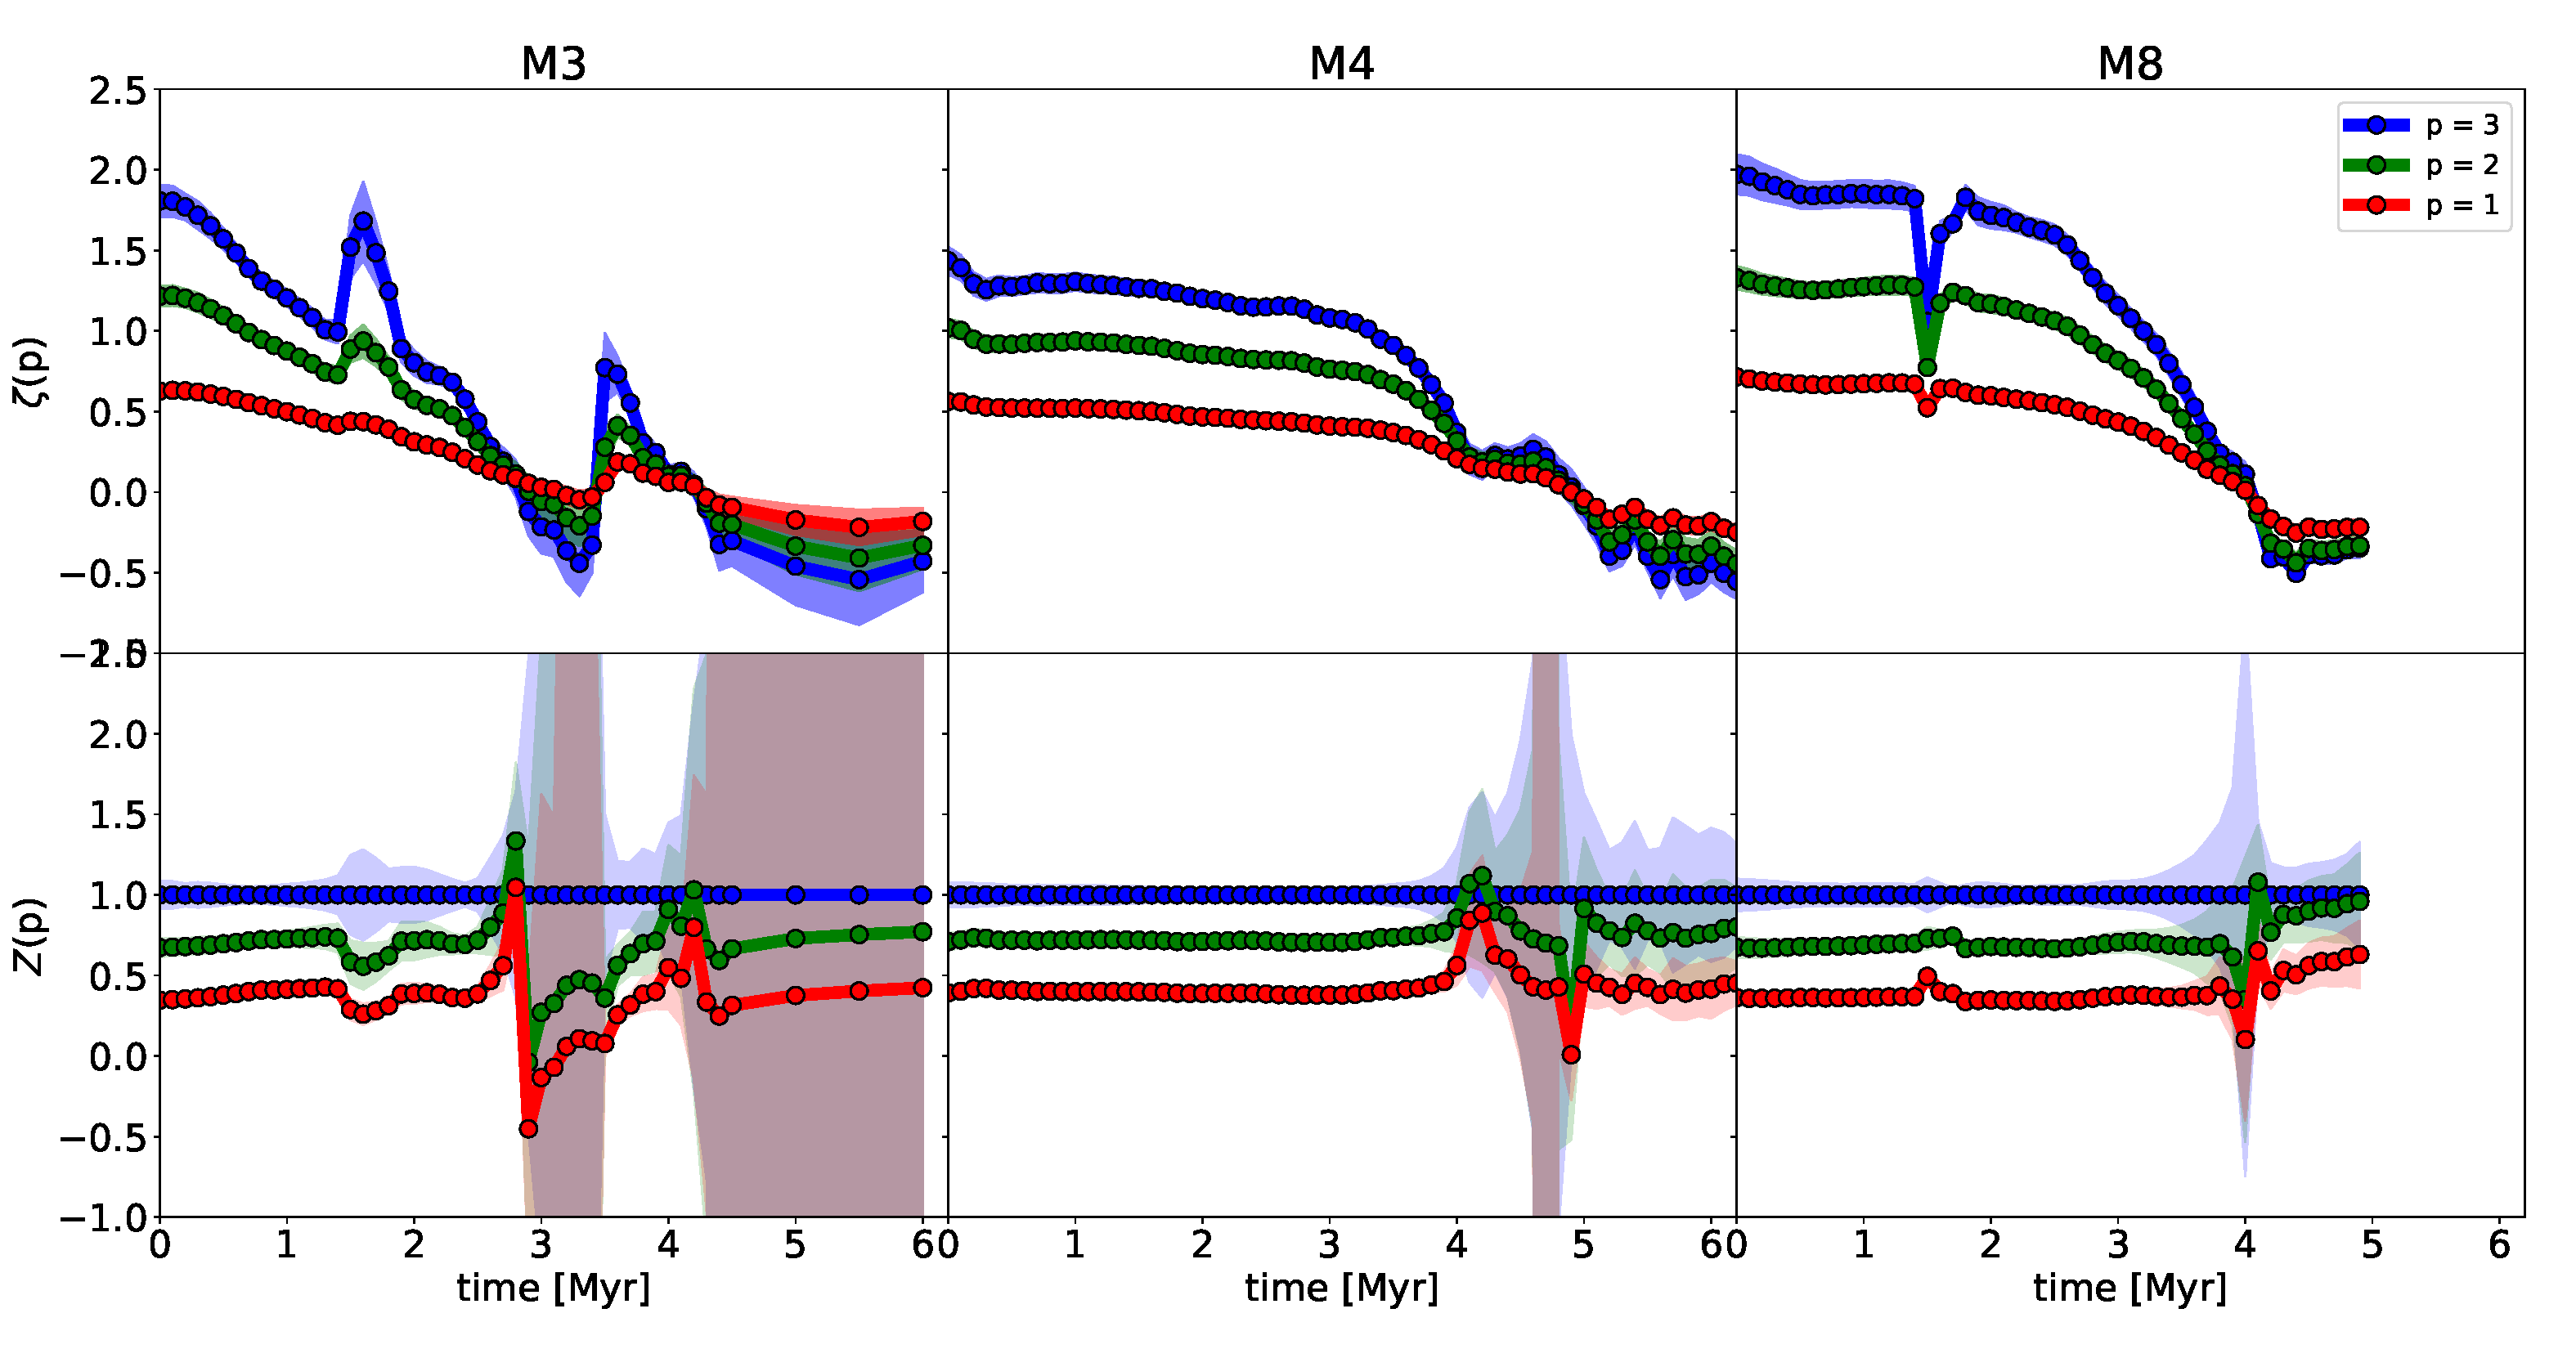
\includegraphics[width=0.9\textwidth]{error_vsf04_zeta_z.pdf}
\caption{
    Data presented in Fig.~\ref{pic:results:zeta_all}a, with
    shaded areas behind the data representing the error ranges of the computed $\zeta$ (\textit{top}) and $Z$ (\textit{bottom}).
}
\label{pic:appFitting:error_vsfhr04_zeta_z}
\end{figure*}


The fit also provides the $\chi^2$ errors for the measured values of $\zeta$. 
In Fig.~\ref{pic:appFitting:error_vsfhr04_zeta_z} we show a reduced version of Fig.~\ref{pic:results:zeta_all}(a), where we only plot the time evolution of $\zeta$ for all three clouds, along with shades of the same colours of the respective lines that represent the errors.
We see that the relative errors, $\Delta \zeta / \zeta$ mostly remain within a range of 5--12\%. 
The errors of $Z$ are computed by Gaussian error propagation
\begin{align}\Delta Z(p) &= \sqrt{ \left( \frac{\partial Z(p)}{\partial \zeta(p)} \cdot \Delta\zeta(p) \right)^2 + \left( \frac{\partial Z(p)}{\partial \zeta(3)} \cdot \Delta\zeta(3) \right)^2 } \\
    &= \sqrt{ \left( \frac{\Delta\zeta(p)}{\zeta(3)} \right)^2 + \left( \frac{ \zeta(p) \cdot \Delta\zeta(3)}{\zeta(3)^2} \right)^2 }.
    \label{equ:appFitting:z_error}
\end{align}
\noindent In general, the relative errors of $Z$ are, as well, around 10\%, though we do see exceptions with very large errors. 
The reason for these is that at these times $\zeta$(3) approaches zero, causing Eq.~(\ref{equ:appFitting:z_error}) to diverge.



\endinput
